\section{Zielsetzung}
Ziel der Versuch ist es die elastischen Konstanten eines Körpers (hier: einer Kugel) zu bestimmen. Anschließend soll das magnetische
Moment eines Permanentmagneten unter Zuhilfenahme eines Helmholtzspulenpaares bestimmt werden.
\section{Theorie}
\label{sec:Theorie}
    \subsection{Normal- und Schubspannung}
    Wenn auf die Oberfläche eines Körpers eine Kraft $F$ wirkt, kann es dabei zu Verformungen und Volumenänderungen am Körper
    kommen. Hier soll $F$ eine Zugkraft sein, das heißt eine Kraft die an der Oberfläche des Körpers zieht. Diese Kraft wird
    als Spannung bezeichnet, wobei die auf der Oberfläche senkrechtstehende Komponente als Normalspannung $\sigma$ bezeichnet wird
    und die Komponente welche parallel zur Oberfläche verläuft als Schubspannung $\tau$.
    Zu Beachten ist dabei aber auch, dass sich die an der Oberfläche wirkenden Kräfte auf den ganzen Körper auswirken.
    Desweiteren wird eine Deformation als elastisch bezeichnet, wenn sich der Körper nach Einwirken einer Kraft wieder in seinen
    ursprünglichen Zustand zurückversetzt, also seine ursprüngliche Form wieder annimmt. Dies gilt bei jedem Körper für einen 
    gewissen Bereich des Zusammenhanges zwischen Kraft $F$ und Deformation (siehe \autoref{sec:hook}). Allgemein lässt sich dieser 
    proportionale Zusammenhang mithilfe von Konstanten beschreiben. Auf die Definition und den Zusammenhang dieser Konstanten wird 
    in \autoref{sec:konstanten} näher eingegangen.
    \subsection{Hook'sches Gesetz}
    \label{sec:hook}
    Das Hook'sche Gesetz gilt solange der Körper nur einer geringen Spannung $\sigma$ ausgesetzt ist, so dass nur eine elatische 
    Deformation vorliegt. Der Aufbau eines Körpers wird dabei
    als Kristallgitter betrachtet, in dem sich die Atome beziehungsweise Moleküle in einem Abstand $r$ in einem 
    Gleichgewicht befinden. Durch Einwirkung einer äußeren Kraft verschiebt sich dieses Gleichgewicht und der Körper deformiert.
    Solange die Spannungen nicht zu groß sind, ist diese Deformation reversibel, sodass sich ein proportionaler Zusammenhang zwischen
    ergibt:
    \begin{equation}
    \label{eqn:hook}
        \sigma = E \frac {\Delta L} {L},
    \end{equation}     
    wobei $\frac {\Delta L}{L}$ die relative Längenänderung der Körpers und E das Elastizitätsmodul, auf welches in \autoref{sec:konstanten}
    näher eingegangen wird, bezeichnet.
    Insgesamt sind für die Beschreibung des Zusammenhanges zwischen Spannung und Deformation in einem Kristallgitter 36 Konstanten
    notwendig, durch Symmetrien veringert sich diese Zahl allerdings erheblich. 
    \subsection{Elastische Konstanten isotroper Körper}
    \label{sec:konstanten}
    Als isotrope Materialien werden Stoffe bezeichnet, deren Elastizitätskonstanten richtungsunabhängig sind. Hierdurch verringert
    sich die Zahl der Konstanten auf zwei.
    Die Konstanten sind einerseits das Schub- beziehungsweise Torsionsmodul $G$, welches die Gestaltselastizität beschreibt, 
    andererseit das Kompressionsmodul $Q$, welches die Volumenelastizität beschreibt. Hinzu kommen, aus Gründen der Zweckmäßigkeit,
    noch das bereits erwähnte Elastizitätsmodul $E$ und die Poisson'sche Querkontraktionszahl $\mu$.
    $E$ beschreibt dabei die Längenänderung des Körpers unter Einfluss einer Normalspannung in Spannrichtung, während $\mu$ 
    die Längenänderung des Körpers senkrecht zur Normalspannung beschreibt. 
    Des Weiteren gelten folgende Zusammenhänge zwischen den Modulen:
    \begin{equation}
    \label{eqn:Zusammenhang1}
    E = 2 G (\mu + 1)
    \end{equation}
    und
    \begin{equation}
    \label{eqn:Zusammenhang2}
    E = 3 (1- 2 \mu) Q.
    \end{equation}
    Hieraus lassen sich die Module direkt berechnen, zu
    \begin{equation}
    \label{eqn:mubestimmen}
    \mu = \frac{E}{2G} -1
    \end{equation}
    und 
    \begin{equation}
    \label{eqn:Qbestimmen}
    Q = \frac{EG}{9G - 3E}
    \end{equation}
\subsection{Bestimmung des Schubmoduls $G$}
    
    $G$ wird durch Betrachtung einer Torsion an einem zylindrischen Körper ermittelt, an dem eine Kraft $K$ an zwei entgegengesetzen 
    Punkten des Körpers wirkt.  
    Das hierdurch entstehende Drehmoment $M$ ruft eine Torsion der unteren Zylinderfläche gegen die obere um den Winkel $\phi$ hervor.
    Bei der Berechnung von diesem, ist allerdings noch die Wirkung der Hebelarme, also dem Abstand der Massepunkte von der Drehachse,
    zu beachten, welcher aber über den Durchmesser des Körpers variert. 
    Mithilfe der Länge $L$ des Körpers und dem aus \autoref{fig:Hohlzylinder} ablesbaren Scherungswinkel $\alpha = \frac{r \phi}{L}$
    ergibt sich unter Berücksichtigung des Hook'schen Gesetzes das Drehmoment
    \begin{equation}
    \label{eqn:drehmoment}
    M = \int_0^{R} 2 \pi \frac{G}{L} r^3 \, dr = \frac {\pi}{2} G \frac {R^4}{L} \phi,
    \end{equation}
    woraus sich ein Proportionalitätsfaktor, die Richtgröße des Zylinders 
    \begin{equation}
    \label{eqn:richtgroesse}
    D := \frac{\pi G R^4}{2L},
    \end{equation}
    ableiten lässt.
    \begin{figure}
        \centering
        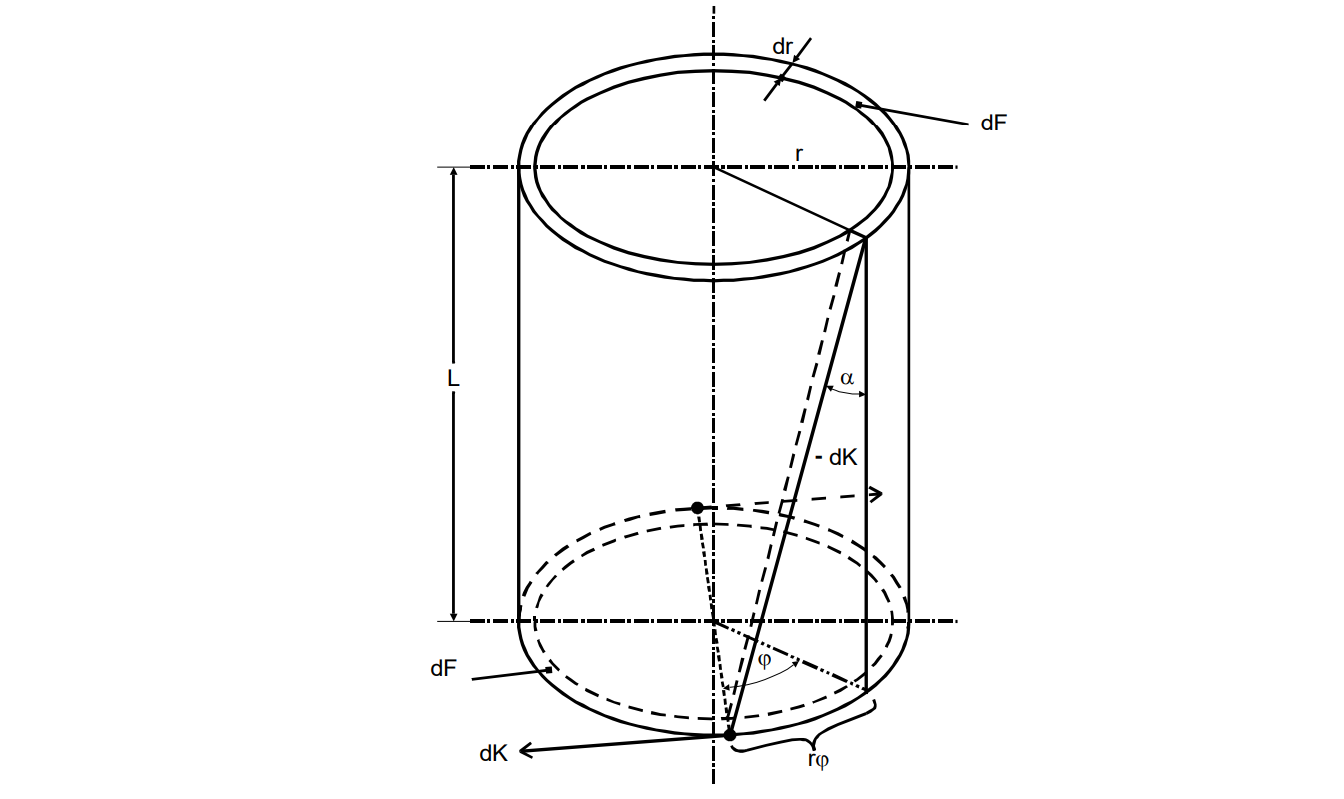
\includegraphics[width=\textwidth]{content/hohlzylinder.png}
        \caption{Schema zur Verdeutlichung des Zusammenhangs zwischen Drehmoment $M$ und Torsionswinkel $\phi$ an einem Zylinder \cite[97]{V102}.}
        \label{fig:Hohlzylinder}
    \end{figure}
    Durch Betrachtung eines Aufbaus an dem eine Kugel an einem (zylinderförmigen) Draht gehängt und ausgelenkt wird, werden sogenannte
    elastische Nachwirkungen umgangen.Es greifen nun zwei entgegengesetzt wirkende Drehmomente,
    einerseits das des Drahtes welches mit Gleichung \eqref{eqn:drehmoment} dargestellt wird
    und andererseits das der Kugel, welches durch die Trägheit der Kugel $\Theta$ hervorgerufen wird: 
    \begin{equation}
    \label{eqn:drehmomentkugel}
    M_K = \Theta \frac{d^2\phi}{dt^2}.
    \end{equation}
    Aus den Gleichungen \eqref{eqn:drehmoment}, \eqref{eqn:richtgroesse} und \eqref{eqn:drehmomentkugel} lässt sich die Bewegungsgleichung
    als Differentialgleichung zweiter Ordnung formulieren:
    \begin{equation}
    \label{eqn:diffgleichung}
    D \phi + \Theta \frac{d^2\phi}{dt^2} = 0 .
    \end{equation}
    Durch Lösen mithilfe eines Cosinus-Ansatzes und des Trägheitmomentes $\theta$ einer Kugel
    \begin{equation}
        \label{eqn:traegheit}
        \theta = \frac{2}{5} m_K R_K^{2}
    \end{equation}    
    ergibt sich die Periodendauer $T$ zu
    \begin{equation}
    \label{eqn:periodendauer2}
    T = 2 \pi \sqrt{\frac{4 m_K R_K^{2} L}{5 \pi G R^4 }},
    \end{equation}
    wobei $m_K$ die Masse und $R_K$ der Radius der Kugel sind.
    Somit lässt sich das Schubmodul $G$ schließlich über Glecihung \eqref{eqn:periodendauer2} bestimmen zu
    \begin{equation}
    \label{eqn:schubmodul}
    G = \frac{16 \pi m_K R_K^{2} L}{5 T^2 R^4}.
    \end{equation}
\subsection{Bestimmung des magnetischen Moments eines Permanentmagneten} 
    \begin{figure}
        \centering
        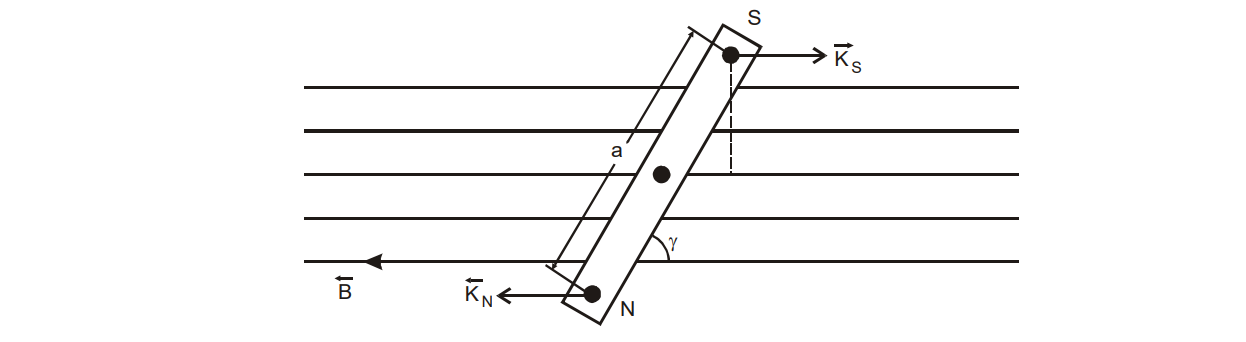
\includegraphics[width=\textwidth]{content/magnet.png}
        \caption{Permanentmagnet in einem äußeren, homogenen Magnetfeld \cite[103]{V102}.}
        \label{fig:magnet}
    \end{figure}
    Das magnetische Moment $\vec{m}$ ist definert als Produkt der magnetischen Polstärke der Pole und dem Abstand $a$ zwischen den Polen
    Durch anlegen eines homogenen Magnetfeldes wirken, zwei Kräfte an den beiden Polen in 
    entgegengesetzter Richtung, sodass ein Drehmoment $M_\text{mag}$ resultiert mit
    \begin{equation}
    \label{eqn:magdrehmoment}
    M_\text{mag} = p \vec{a} \times \vec{B} = \vec{m} \times \vec {B}.
    \end{equation}
    Wenn derselbe Aufbau wie zur Bestimmung des Drehmomentes genutzt 
    wird kann die Differentialgleichung \eqref{eqn:diffgleichung} zu
    \begin{equation}
    \label{eqn:magdiff}
    m B \sin \phi + D \phi + \Theta \frac{d^2\phi}{dt^2} = 0 
    \end{equation}
    aufgestellt werden.
    Lösen der Differentialgleichung ergibt eine Periodendauer von
    \begin{equation}
    \label{eqn:Periodendauermagnet}
    T_m = 2 \pi \sqrt{\frac{\Theta}{m B + D}}.
    \end{equation}

